\chapter{Modular Anomaly Detection Framework}
\label{chapter:Chapter 3}
\lhead{Chapter 3. \emph{Methods and Systems Developed}}

In this Chapter, we present the overall description of steps towards the development of the \emph{Modular Anomaly Detection Framework} which will be used throughout this thesis. 
A crucial component in this work relied on a technically accurate definition of a \emph{maritime anomaly}. This is generally speaking a challenging task since a data-driven definition is currently lacking or insufficient. A more meaningful solution to this problem was provided by the aid of maritime experts who were engaged in the \textsc{marisa} project. In particular, members of the Portuguese Navy interacted with us in order to offer the required their exclusive technical insight.

Given their specific input and real-world knowledge of the maritime domain, one can arrive at a well-defined concept of anomaly that can be translated into a precise notion to be used in this Framework. Before we engage in the specific requirements that served as a blueprint for the developed framework, such a definition will be given. This will then be followed by the technical description of such requirements, namely by distinguishing \emph{anomaly} and \emph{data requirements}.

Lastly, a general overview of the proposed Modular Anomaly Detection Framework, which will be referred to as MAD-F from now on, is presented. This is done in light of Figure \ref{fig:Framework}, whose modules are explained individually throughout the following Subsections \ref{subsection: Data Ingestion}, \ref{subsection: 3 Pre-processing}, \ref{subsection: 3 Feature Engineering},  \ref{subsection: 3 Vessel Trajectory Extraction}, \ref{subsection: 3 ADS} and \ref{subsection: 3 RB-ADS}.


\section{Anomalies within the Framework}
\label{section: Framework Requirements}
An anomaly may have numerous interpretations depending on the context in which it is found. However, it can be generally conceptualised as a subset of data that stands out in some preconceived way when contrasted to the overall dataset. Nowadays, the anomaly detection of vessel behaviour is solely done by human maritime experts. This procedure depends on national security agencies. Within their duties, these agencies are responsible for assuring the coastal surveillance of their territory by assessing possible threats and identifying abnormal behaviour. The current methods employed by these institutions are neither efficient nor scalable and therefore not suitable for the challenges brought by the exponential growth of vessels at seas. This state of affairs creates an ideal situation for the use of data-driven models to assist the maritime experts.

The notion of anomaly just presented is unsatisfactory given both the complexity and purpose of the problem. For the goals of this project, such a technical definition is tailored specifically by the maritime agencies involved in the \textsc{marisa} project and we therefore refrain from applying our own definitions, which usually stem from abstract statistical data-driven notions. 

By having meetings with maritime experts a list of the anomaly requirements was agreed. For this work this list served as not only the concrete anomaly requirements, but also as a guide for the overall implementation of the \emph{MAD-F}. The list of anomaly requirements in shown under in Table \ref{Table: Anomaly Requiremtens}.

\begin{table}[H]
\centering
\caption{MAD-F anomaly requirements, which were defined by maritime officers.}
\label{Table: Anomaly Requiremtens}
\begin{tabular}{@{}ll@{}}
\toprule
Anomaly Requirement & Provided Description \\ \toprule
\textit{\textbf{AR1}} & \begin{tabular}[c]{@{}l@{}}Detect Abnormal changes of \\ (more than a configurable value) Direction.\end{tabular} \\ \midrule
\textit{\textbf{AR2}} & \begin{tabular}[c]{@{}l@{}}Detect Abnormal changes of \\ (more than a configurable value) Velocity.\end{tabular} \\ \midrule
\textit{\textbf{AR3}} & \begin{tabular}[c]{@{}l@{}}Detect Vessels disappearance from sensor \\ coverage for more than a configurable Time Period.\end{tabular} \\ \midrule
\textit{\textbf{AR4}} & \begin{tabular}[c]{@{}l@{}}Detect when the observed \\ Vessel Navigational Status is not consistent \\ with the reported Vessel Kinematic features.\end{tabular} \\ \midrule
\textit{\textbf{AR5}} & \begin{tabular}[c]{@{}l@{}}Detect when Vessels report a \\ geographical and time incompatibility.\end{tabular} \\ \midrule
\textit{\textbf{AR6}} & \begin{tabular}[c]{@{}l@{}}Detect when two or more Vessels are \\ approaching close to each other.\end{tabular} \\ \bottomrule
\end{tabular}
\end{table}

As mention previously, requirements for this work were distinguished from anomaly requirements and data requirements. The latter was intrinsic for this work, as the uncertainty of data types and sources when dealing with the maritime field is immense. The problem of having numerous types and sources of data is still aggravated as the maritime domain is also capable to produce enormous workflows of data. Thus, a specific data requirement for this work could be simply specified as: 

\emph{The developed Framework, must be able to ingest fuse and store different sources of maritime Data, while also handling enormous workflows of data in real-time.}

\section{Modular Vessel Anomaly Detection Framework}
In order to develop a Framework capable of achieving the requirements defined above in \ref{section: Framework Requirements}, we propose the Modular Vessel Anomaly Detection Framework. The \emph{MAD-F} is able to ingest data from different feeds in real-time data while simultaneously constructing a Data-Base for Vessels Trajectories in a unsupervised manner. Anomalies are then detected in a offline manner from the saved trajectory data, or online in real time addressing the incoming streams of Vessel Data. 
The framework was developed to be modular as there are either no inputs or outputs standards for the Maritime Domains. Thus, by providing a configurable and not static framework, we give the configuration flexibility for the \emph{MAD-F} being configured for different scenarios or even different National Maritime Authorities, or even to new Modules being added in the future.
In Figure \ref{fig:Framework} we present the architecture of the \emph{MAD-F} and the following subsections will discuss each of the framework modules: Data Ingestion, Data Pre-processing, Feature Engineering, Trajectory Extraction and both anomaly detection modules : Anomaly Detection Service and Rule Based Anomaly Detection Service.
\todo[inline]{Fix the trajectory extraction module image.}
\begin{figure}[H]
\centering
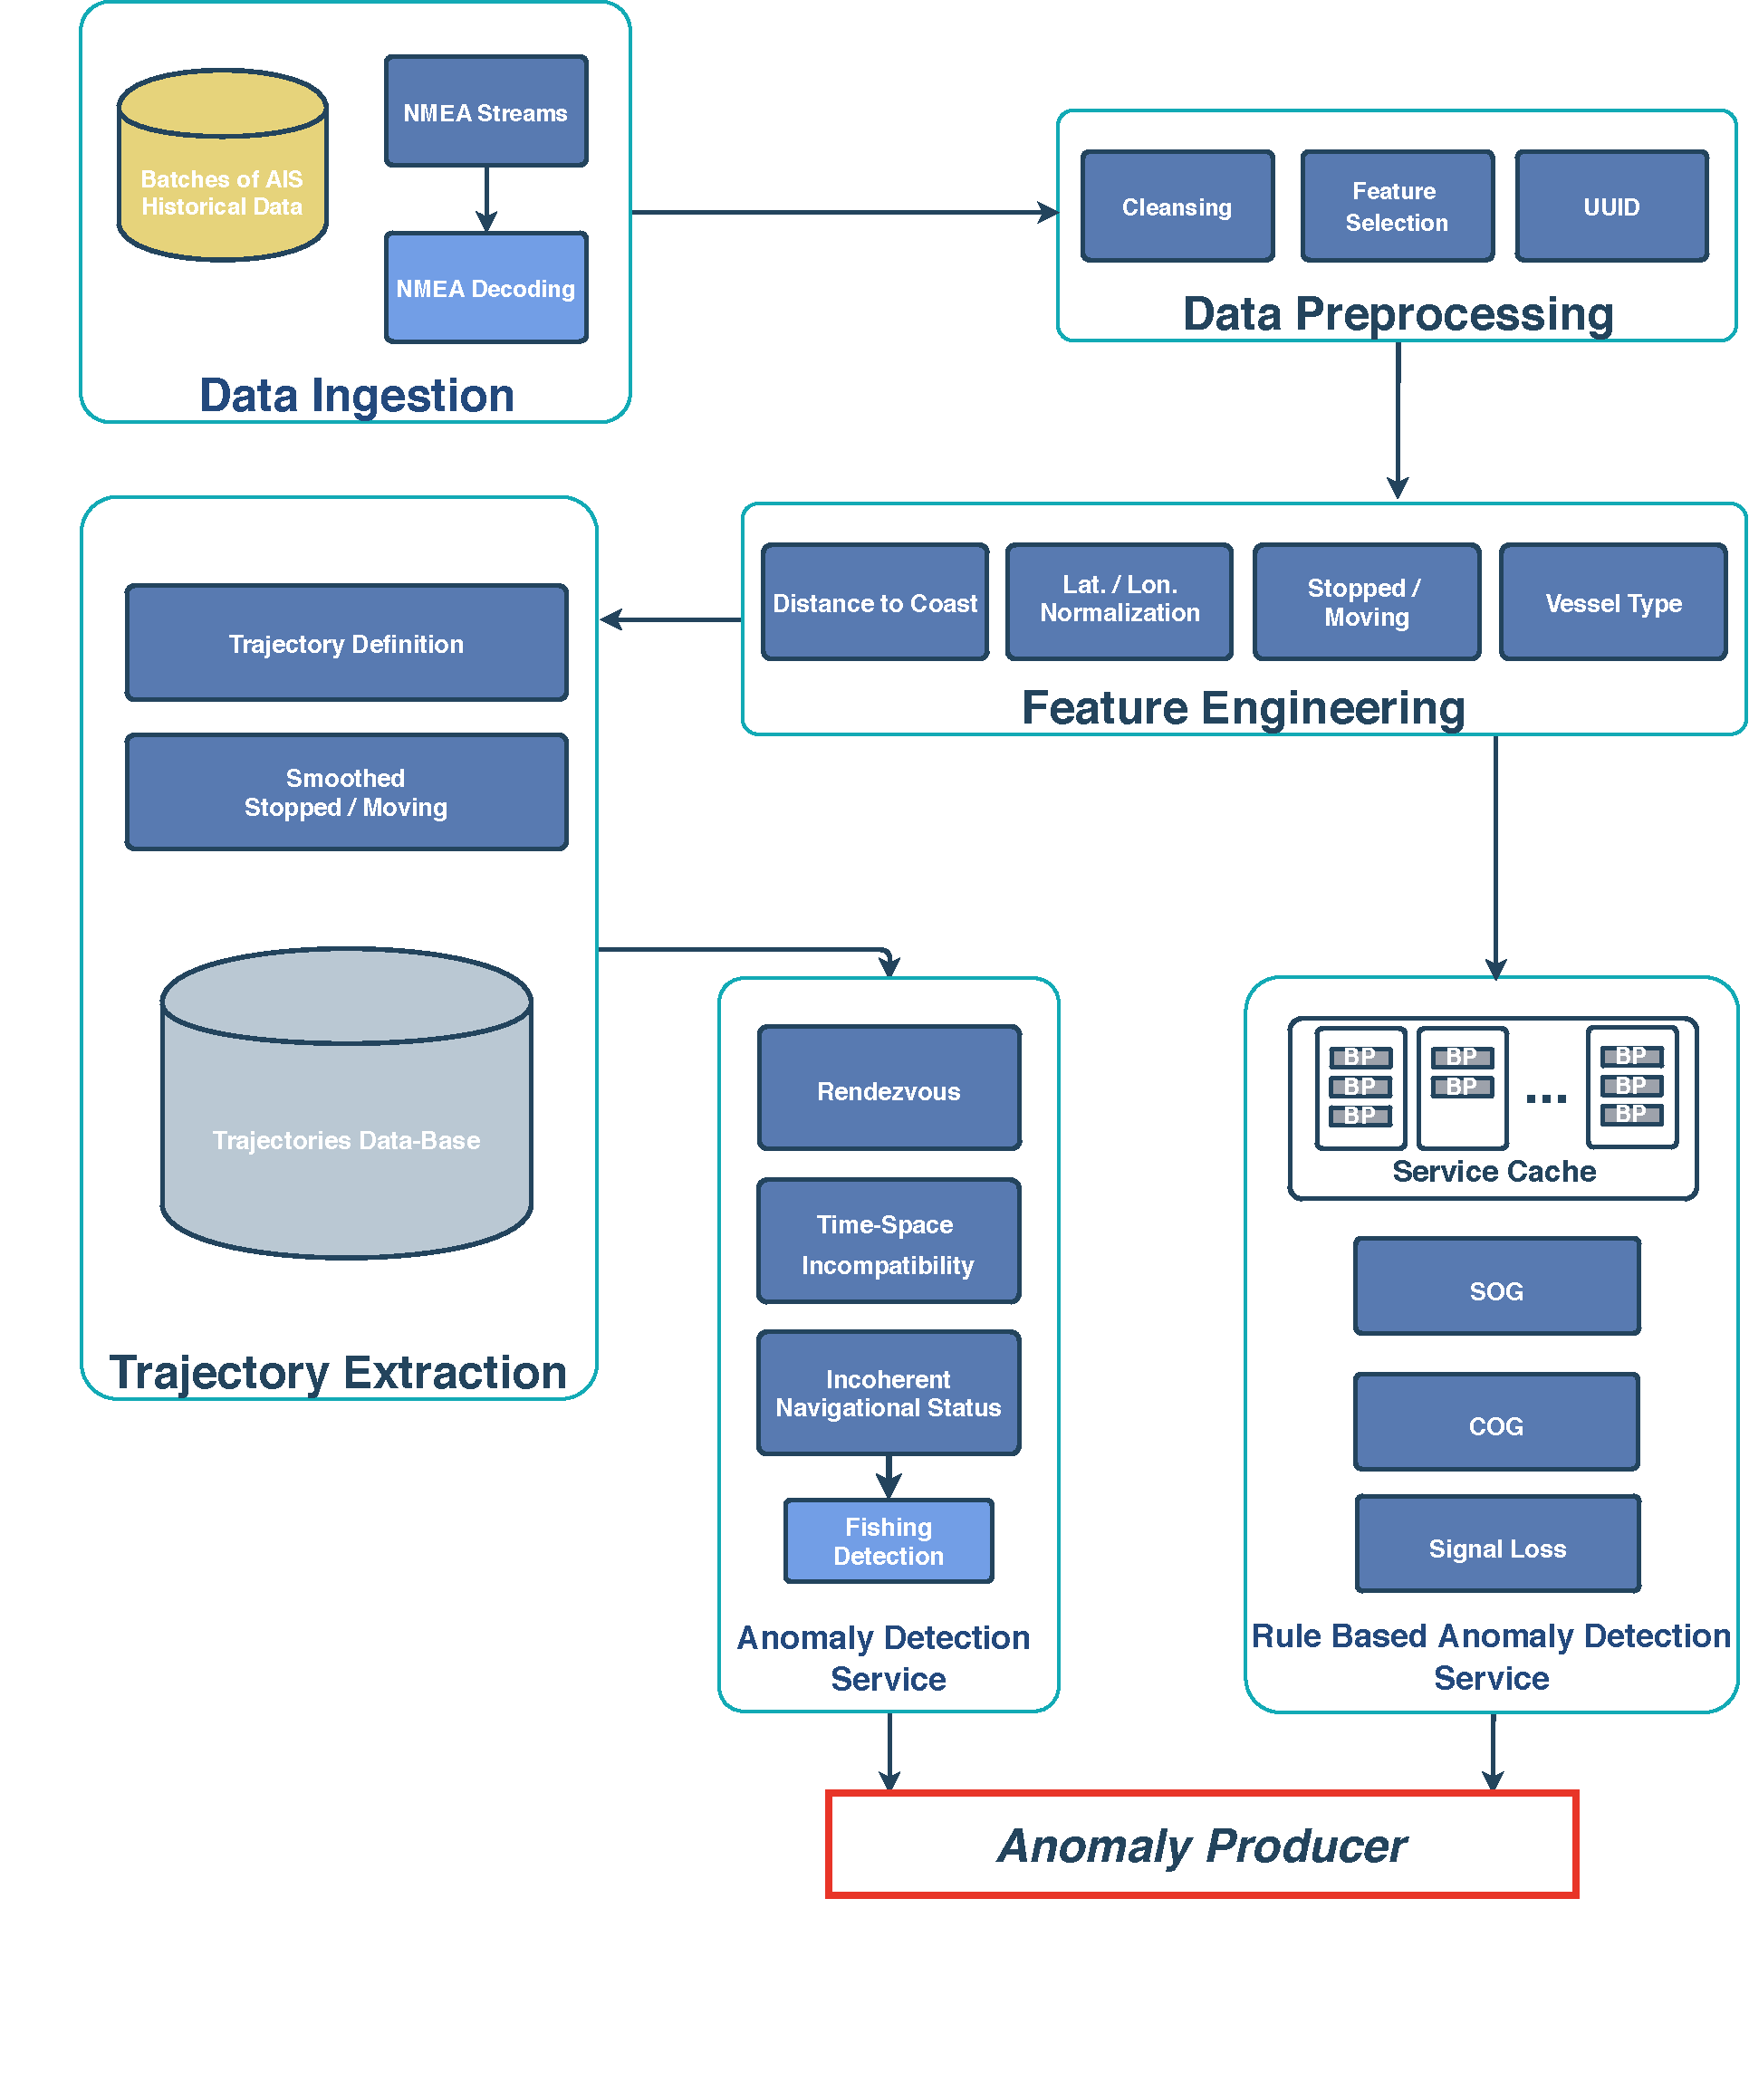
\includegraphics[width=\textwidth]{figures/Ch3/Framework.pdf}
\caption{Proposed architecture for the \emph{MAD-F} Framework}
\label{fig:Framework}
\end{figure}

\subsection{Data Ingestion}
\label{subsection: Data Ingestion}
Data Ingestion Module, represents the Data input for the developed Framework. AIS data was the most representative data type used for this work, as it showcases the actual instantaneous Vessel information.
Although, used AIS data for this work came in two really distinct formats. It came either in \emph{Historical Batches} representing Historical sets of Data, or real \emph{NMEA AIS Streams} which represent real, real-time data. For both data formats, the framework is scalable, and able to ingest one or multiple feeds / sources of data simultaneously.

%AIS Historical Data-Sets, can be found in open-access repositories, although Historical AIS Data providers cap the frequency of the messages transitions. This drastically reduces the number of transmitted messages, but also reduces the overall detail of the Data, as lower transmissions rates produce a less certainty of the movement presented by each Vessel. Which, for most general uses of AIS (e.g. managing a fleet, estimations of time of arrival ...), transmissions rates of 3 Seconds vs 30 Seconds, do not provide any information gain, as Vessel kinematics tend to not change abruptly in short periods of time. 

Via the MARISA project, we accessed AIS live feeds from antennas all around the Portuguese coast line. This Antennas receive Vessels transmissions via AIS up to 20 Nautical Miles of the shore depending on the weather conditions, and with reception rates up to 30 Messages per minute per vessel. The real live feeds of AIS data, are received via TCP in the NMEA format.

National Marine Electronics Association (NMEA) is a standard communication protocol used by Maritime Sensors such as Accelerometer, Giroscope, GPS receivers, etc.
NMEA encapsulates the information from the different Vessel sensors, and broadcasts this information to coastline antennas and nearby Vessels via AIS protocol.

\begin{figure}[H]
\centering
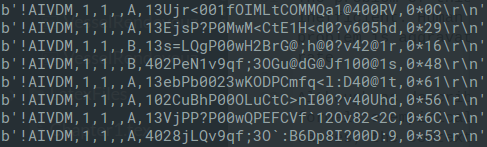
\includegraphics[scale = .5]{figures/Ch3/NMEAexample.png}
\caption{Snapshot of raw AIS data in NMEA format.}
\label{fig:NMEAexample}
\end{figure}
\todo[inline]{This Needs a new IMAGE message.}
%Via the project, we had access to multiple live NMEA feeds, as a way to not only validate our developed methods with live feeds of Nautical data, but also to produce methods that were capable of handling the scale of data that is produced by National feeds.
Although the use of real AIS data comes with many challenges, as it is mandatory to decode, sort and store the received data, thus allowing the incoming data to be used as viable source of data. Secondly, as AIS-receiving stations receive the broadcast AIS information from multiple AIS-equipped vessels simultaneously, and the reception range of each AIS-receiving can vary depending on the actual weather conditions and the location of where such station is located. This originates two main problems :
\begin{enumerate}
\item Duplication of reception:  With the variation of reception ranges from the AIS-receiving stations, this creates the problem of multiple stations receiving the same vessel broadcast. The duplication of messages is a problem which occurs when handling real NMEA streams, the methods used to solve such problem are presented in Section XX.

\item Non-reception of broadcast: Similar to the problem presented above the non-reception of by any receiving station can also occur. To address this problem, Maritime Agencies use satellite AIS (S-AIS). S-AIS solves the problems related to the reception range, but presents another problem with refreshment rates, has the reception of the broadcast are dependent of satellite revisit time \cite{Robards2016ConservationReview}. 
\end{enumerate}


%when dealing with real-time NMEA feeds as
%the reception range of the AIS receiving antennas varies depending on weather condition when this antennas receive information from multiple Vessels two more common problems can occur:


%. Normally, AIS-Receiving stations are antennas located along the coast line in high grounds, the reception range of these antennas vary, mainly depending on distance to shore, the elevation in which the antenna is located, and the antenna type itself.

%Although, the distance in which Stations are capable of receiving AIS messages presents a problem to the Data, as reception ranges vary from 15 Nautical Miles to 50 Nautical Miles, which creates the problem of 



%\subsection{Data Storage}
%With NMEA streams producing enormous workflows of data, the storage of becomes a problem for the developed Framework, as it must not only decode and process the NMEA feeds but also store the decoded messages, in a "very fast" and scalable way.

%Thus, and as requirement of the MARISA project was to use Apache Spark [REF FOR APACHE SPARK] modules for data-ingestion and pre-processing, we decided to use Apache Cassandra as the Data-Storage for the proposed framework.

\subsection{Data Pre-processing}
\label{subsection: 3 Pre-processing}
The Data Pre-processing module, is the first step of Data Wrangling in our Framework, the motive for this module is to select, transform, and clean the received data, incoming from the Data Ingestion Module. 
As described in Section \ref{subsection: chp2_AIS}, AIS presents a large amount of different features, which can be used for different problems. Feature Selection represents a important step for this work. This work being partially a unsupervised learning problem, the selection of the "relevant" features directly influences the overall performance of the \emph{MAD-F}, but also the expected results from the learning task. Such representative task requires pre-conceived knowledge of Vessels dynamics and behaviour, which is only gained with experience in the Maritime Domain. For this work the feature selection was done based on the literature, and also by accessing Maritime Expert Knowledge via the MARISA project.

During the \emph{Pre-processing}, a data-cleaning process is conducted, discarding corrupted data. This is done based on the information that standardises the AIS features, which is further detailed in Section~\ref{section: Data Analysis}.

Most importantly, in this module the concept of \emph{Behavioural Point} is defined. \emph{Behavioural Point} which will be referred as $BP$ from now on, for this work represents our normalised representation of the previously selected features. A detailed explanation of this concept is provided in Subsection \ref{subsection: Behavioural Point}.

\subsection{Feature Engineering}
\label{subsection: 3 Feature Engineering}
Feature Engineering, represents the second step of Data Wrangling for the proposed Framework. During this step, the already pre-defined $BPs$, in the Data Pre-processing module, are enriched by extrapolating additional features. 

Firstly for each $BP$ received by this module, if the Vessel Type is not received in the AIS message, the Vessel Type is either extracted from external Vessel Information Sources, or it is scrapped from this internet.
Secondly, each $BP$ is enriched with by calculating the closest country and respective distance to Shore. The same is done to Ports, by calculating the distance to the closest Port. Also, in this module with the reported kinematic features, the instantaneous move state of the vessels is inferred.

This procedures are further individually explained throughout Subsections \ref{subsection: Vessel Type}, \ref{subsection: Distance to Coast}, \ref{subsection: Stopped/Moving}.

%presents a crucial step for any machine learning project, as 

%selecting the right features to represent the data, directly influences any result generated by the Anomaly Detection Modules.  

%We further enrich our features in two ways, firstly by analysing each AIS message as a single point in Time and calculating additional distances, such as distance to Shore and distance to the most near Port.

%each point in t the represented features of each message by by doing a point based analysis, in which we considered the information of  

%by normalizing the Latitude and Longitude features of each position, calculating the Distance to Shore and the kinematic features that represent the instantaneous move-state of the Vessel. Every calculation is done a priory, thus enhancing the performance and reliability of the Anomaly Detection Modules, which are explained in detail in section \todo{REF TO SECTION!}

\subsection{Vessel Trajectory Extraction}
\label{subsection: 3 Vessel Trajectory Extraction}

Vessel Trajectory Extraction module, handles the definition, storage,  updating and inserting of new incoming $BPs$ into defined \emph{Trajectories}.
When considering Trajectories, the $BPs$ stop being valued as single points in Time, and the aggregation of $BPs$ via the Vessel Identifier throughout time, start representing a Vessel Trajectory. This allows a more conclusive Vessel behaviour analysis based on its past trajectory. Although, in order to work with Trajectory, such concept needs to be defined and represented in a optimal manner. Furthermore, when dealing with real Maritime data (and specially when working with real Maritime Authorities) it is extremely important to trace-back/log of the data, from which, justifying generated anomalies is possible. 
In Section \ref{subsection: Trajectory Definition} our definitions of a vessel trajectory. 

%Behaviour analysis based on the past historical Trajectory data. Analysis of Trajectories drastically increases the level of complexity, when compared to analysis points, thus it is required quick and efficient representation of a Trajectory.

\subsection{Anomaly Detection Service}
\label{subsection: 3 ADS}
ADS (Anomaly Detection Service) Module, represents for our Framework the Batch Layer for Anomaly Detection Services. \emph{ADS} module works offline in effective time, on batches of historical Trajectory Data served from \emph{Trajectory Data-Base} from the \emph{Trajectory Extraction} module. Access to Trajectory Data, is done by querying the \emph{Trajectory Data-Base} with a configurable set of parameters, which can be time restrictive(such as the 10 past Hours) and or from a Vessel specific set of Vessels. 

Received Trajectory Data, is then used to detect: \textbf{Time Space Incompatibility}, \textbf{Vessels Rendezvous}, and \textbf{Incoherent use AIS Navigational Status}. For the latter, we create a sub-method for the detection of \textbf{Fishing Activities} based on Vessels characteristics and Dynamics and the reported Navigational Status.
The implemented methodology for the detection of each Anomaly is represented in Subsections \ref{subsection: 4 Time-Space Incompatibility}, \ref{subsection: 4 Navigational Status Validation}, \ref{subsection: Fishing Activity Detection} and \ref{subsection: 4 Vessel Rendezvous} respectively.


\subsection{Rule Based - Anomaly Detection Service}
\label{subsection: 3 RB-ADS}
RB-ADS (Rule Based - Anomaly Detection Service), opposed to the ADS module described above, corresponds to the Speed Layer for the Anomaly Detection Services. \emph{RB-ADS} modules works online in near real-time, accessing the stream of already pre-processed $BPs$ from the Feature Engineering Module. In order to the \emph{RB-ADS} be able to perform Anomaly Detection in near real-time, a Queuing Systems for this module was defined, which we named \emph{Service Cache}, which we further explain in Section \ref{section: 4 Rule Based Anomaly Detection}. The arriving stream of $BPs$, is are stored in individual Vessel Queues of size $N$. The individual Queues are then accessed, allowing a real-time calculation of the set of Anomaly which can be defined by Rules. The Anomalies validated online trough rules for this work are: Abnormal change of Velocity and Direction (Anomaly Requirements 1 and 2 respectively) and Vessel Signal Loss (Anomaly Requirement 3), our approach towards the detection of such anomalies is described in Section \ref{subsection: 4 Course}  


%This was if i talked about AIS SIGNAL LOOS HERE
%Ships equipped with AIS are obliged to keep the AIS autonomously transmitting AIS messages. A way that ships illegally hide their position and possible what the ships is doing objectively, is by switching off the AIS, or finding ways to block the communications of the AIS transmitter with the coastal receivers.

%This creates a problem in the maritime domain, has maritime authorities are constantly finding new ways to discover this illegal activities. A method that looks into historical or new streams of data, was developed. 

%\subsection{Time Series Analysis}

\subsection{Anomaly Producer}
Anomaly Producer, serves for this Framework as exit point for the MAD-F.This module communicates with other outside services by producing anomalies generated by the Anomaly Detection modules from the Framework. As for this present work, due to the Marisa duties we did not develop any anomaly visualisation module. This module produces anomalies, in the normalised MAD-F anomaly format which we will discuss in Section XX.
